\documentclass{beamer}\usepackage[]{graphicx}\usepackage[]{color}
%% maxwidth is the original width if it is less than linewidth
%% otherwise use linewidth (to make sure the graphics do not exceed the margin)
\makeatletter
\def\maxwidth{ %
  \ifdim\Gin@nat@width>\linewidth
    \linewidth
  \else
    \Gin@nat@width
  \fi
}
\makeatother

\definecolor{fgcolor}{rgb}{0.345, 0.345, 0.345}
\newcommand{\hlnum}[1]{\textcolor[rgb]{0.686,0.059,0.569}{#1}}%
\newcommand{\hlstr}[1]{\textcolor[rgb]{0.192,0.494,0.8}{#1}}%
\newcommand{\hlcom}[1]{\textcolor[rgb]{0.678,0.584,0.686}{\textit{#1}}}%
\newcommand{\hlopt}[1]{\textcolor[rgb]{0,0,0}{#1}}%
\newcommand{\hlstd}[1]{\textcolor[rgb]{0.345,0.345,0.345}{#1}}%
\newcommand{\hlkwa}[1]{\textcolor[rgb]{0.161,0.373,0.58}{\textbf{#1}}}%
\newcommand{\hlkwb}[1]{\textcolor[rgb]{0.69,0.353,0.396}{#1}}%
\newcommand{\hlkwc}[1]{\textcolor[rgb]{0.333,0.667,0.333}{#1}}%
\newcommand{\hlkwd}[1]{\textcolor[rgb]{0.737,0.353,0.396}{\textbf{#1}}}%
\let\hlipl\hlkwb

\usepackage{framed}
\makeatletter
\newenvironment{kframe}{%
 \def\at@end@of@kframe{}%
 \ifinner\ifhmode%
  \def\at@end@of@kframe{\end{minipage}}%
  \begin{minipage}{\columnwidth}%
 \fi\fi%
 \def\FrameCommand##1{\hskip\@totalleftmargin \hskip-\fboxsep
 \colorbox{shadecolor}{##1}\hskip-\fboxsep
     % There is no \\@totalrightmargin, so:
     \hskip-\linewidth \hskip-\@totalleftmargin \hskip\columnwidth}%
 \MakeFramed {\advance\hsize-\width
   \@totalleftmargin\z@ \linewidth\hsize
   \@setminipage}}%
 {\par\unskip\endMakeFramed%
 \at@end@of@kframe}
\makeatother

\definecolor{shadecolor}{rgb}{.97, .97, .97}
\definecolor{messagecolor}{rgb}{0, 0, 0}
\definecolor{warningcolor}{rgb}{1, 0, 1}
\definecolor{errorcolor}{rgb}{1, 0, 0}
\newenvironment{knitrout}{}{} % an empty environment to be redefined in TeX

\usepackage{alltt}

\usepackage{fontspec}
\usepackage[english]{babel}
\IfFileExists{upquote.sty}{\usepackage{upquote}}{}
\begin{document}



\begin{frame}[label=diagram_rem]
  \frametitle{Schematic diagram of the REM}
  %%

  % \begin{columns}[t]

  %   \begin{column}{0.7\textwidth}
  
\begin{knitrout}
\definecolor{shadecolor}{rgb}{0.969, 0.969, 0.969}\color{fgcolor}
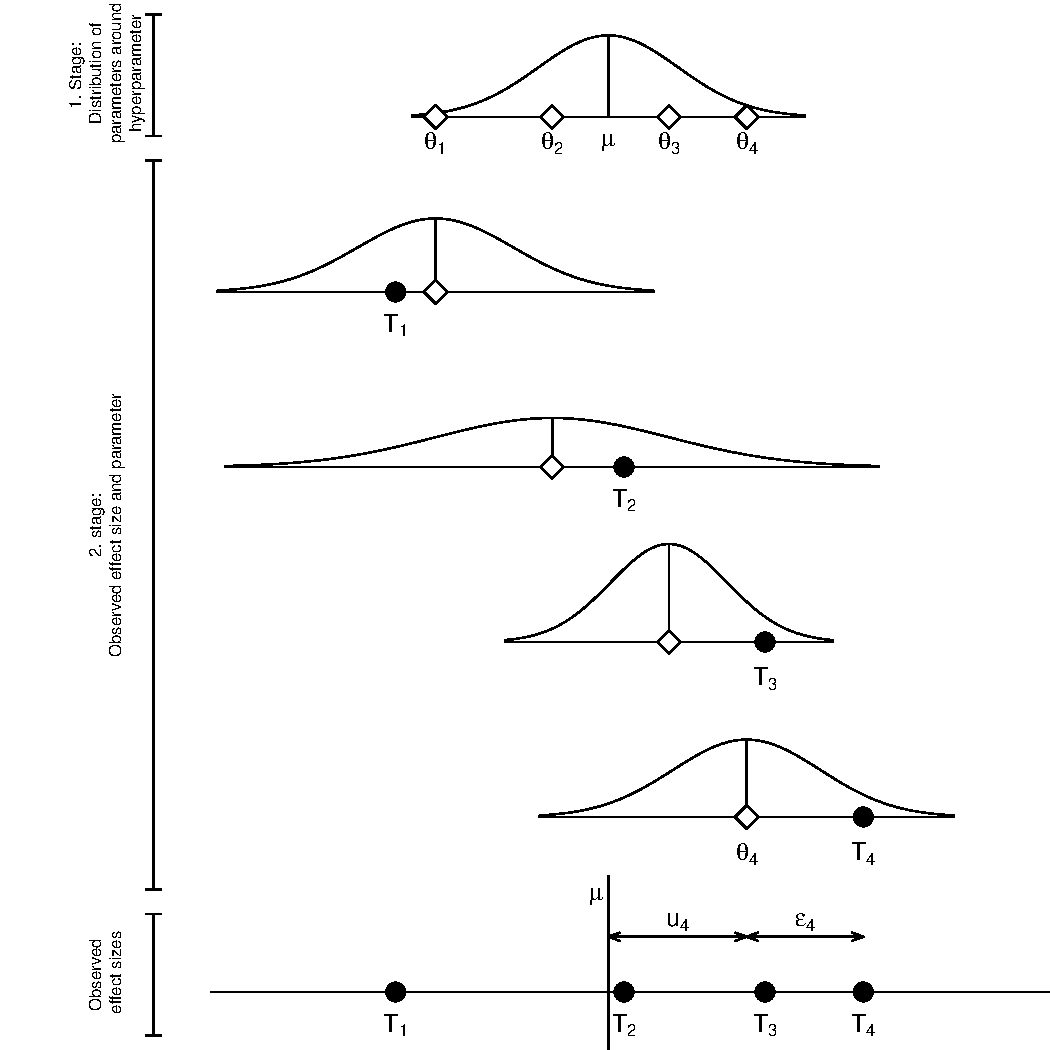
\includegraphics[width=.7\linewidth]{fig/fem_rem_scheme-1} 

\end{knitrout}
\end{frame}


\begin{frame}
  \frametitle{Random-effects model}
  %%
  \begin{itemize}
  \item The random-effects model acknowledges two sources of variation:
    \begin{enumerate}
    \item within-study sampling error ($\sigma_{i}^2$ ) and 
    \item between-studies variability ($\tau^2$) (e.g., due to varying study characteristics).
    \end{enumerate}
    The random-effects model can be represented as
    
    \begin{equation}\label{rand}
      T_i = \overbrace{\mu + u_i}^{\theta_i} + e_i ,
    \end{equation}
    
    % \noindent and the variance of $T_i$ is equal to $\sigma_{i}^2 + \tau^2$ .
    
  \item where
    \begin{itemize}
    \item $e_i$ is the differences between the true mean $\theta_i$ for study $i$ and the
      observed mean effect size $T_i$ for study $i$ ($e_i = T_i - \theta_i$) and 
    \item $u_i$ is the difference between the grand mean $\mu$ and the true mean
      for $i$th study $\theta_i$ ($u_i = \theta_i - \mu$).
    \end{itemize}

\item $e_i$ $\sim$ $N(0,\sigma_{i}^2)$
\item $u_i$ $\sim$ $N(0,\tau^2)$
\end{itemize}
\end{frame}



\begin{frame}
  \frametitle{Random-effects model}
  %%
  \begin{itemize}
  \item Under random-effects model we have two goals:
    \begin{itemize}
  \item To estimate the mean population effect size from which the observed studies are sample from.
  \item To estimate the between-studies variability ($\tau^2$).
\end{itemize}
  \item Although in practice we compute $\sigma_{i}^2$, we treat the within-study error variance as known.
  \item Thus, under random-effects model the variance of $T_i$ is equal to $\sigma_{i}^2 + \tau^2$ .
  \end{itemize}
\end{frame}


\begin{knitrout}
\definecolor{shadecolor}{rgb}{0.969, 0.969, 0.969}\color{fgcolor}\begin{kframe}
\begin{alltt}
\hlkwd{library}\hlstd{(metafor)}
\end{alltt}


{\ttfamily\noindent\itshape\color{messagecolor}{\#\# Loading required package: Matrix}}

{\ttfamily\noindent\itshape\color{messagecolor}{\#\# Loading 'metafor' package (version 2.0-0). For an overview \\\#\# and introduction to the package please type: help(metafor).}}

{\ttfamily\noindent\itshape\color{messagecolor}{\#\# \\\#\# Attaching package: 'metafor'}}

{\ttfamily\noindent\itshape\color{messagecolor}{\#\# The following objects are masked from 'package:meta':\\\#\# \\\#\#\ \ \ \  baujat, forest, funnel, funnel.default, labbe, radial,\\\#\#\ \ \ \  trimfill}}\end{kframe}
\end{knitrout}

\begin{frame}
  \frametitle{Example}
  %% 
  \vspace{-5ex}
\begin{knitrout}\tiny
\definecolor{shadecolor}{rgb}{0.969, 0.969, 0.969}\color{fgcolor}
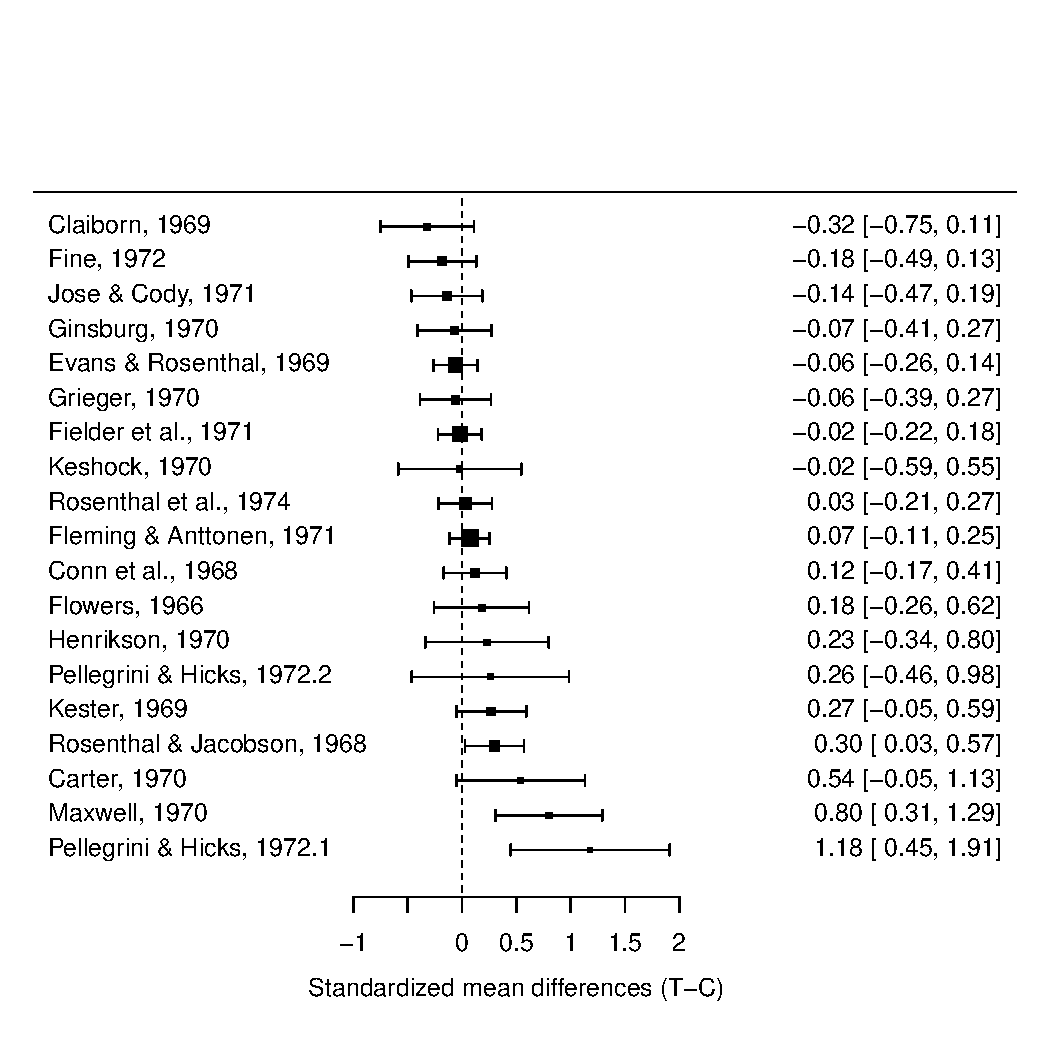
\includegraphics[width=.91\linewidth]{fig/f_forestplot_raudenbush1984-2-1} 

\end{knitrout}
\end{frame}


\end{document}
